 \documentclass[24pt, a0paper, portrait, margin=0mm, innermargin=15mm,
     blockverticalspace=15mm, colspace=15mm, subcolspace=8mm]{tikzposter} %Default values for poster format options.

% to turn off the ad. for the class 
\tikzposterlatexaffectionproofoff

 % Title, Author, Institute
 \title{Using tikzposter}
 \author{Pascal Richter, Elena Botoeva, Richard Barnard, \& Dirk Surmann}
 \institute{}

% Our block style has sharp corners, easier to edit later in Inkscape
\defineblockstyle{Rectangle}{
    titlewidthscale=1, bodywidthscale=1, titleleft,
    titleoffsetx=0pt, titleoffsety=0pt, bodyoffsetx=0pt, bodyoffsety=0pt,
    bodyverticalshift=0pt, roundedcorners=0, linewidth=0pt, titleinnersep=1cm,
    bodyinnersep=1cm
}{
    \ifBlockHasTitle%
        \draw[draw=none, left color=blocktitlebgcolor, right color=blockbodybgcolor]
           (blocktitle.south west) rectangle (blocktitle.north east);
    \fi%
    \draw[draw=none, fill=blockbodybgcolor] %
        (blockbody.north west) -- (blockbody.south west) --
        (blockbody.south east) -- (blockbody.north east) -- cycle;
}

% see original tikzposter example for the options
\usetheme{Autumn}
\usecolorstyle[colorPalette=BrownBlueOrange]{Germany}
\useblockstyle[bodyinnersep=1cm]{Rectangle}

 \begin{document}

     \maketitle

     \begin{columns}%blocks will be placed into columns
         \column{.50}

%%%%% First block %%%%%%

         \block{Creating the document}{
           Content for first block
Want to leave some space for a figure later ?
% just use vspace
\vspace{20cm}

         \begin{tikzfigure}[A figure can be made with \textbackslash\texttt{tikzfigure}; \textbackslash\texttt{figure} does not work]
      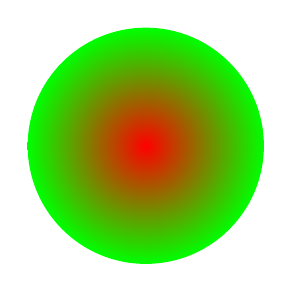
\begin{tikzpicture} % replace by the correct figure
        \draw[draw=none,inner color=red, outer color=green] (0,0) circle (1.5cm);
      \end{tikzpicture}
         \end{tikzfigure}

     }

%%%%% Second block %%%%%

     \block{The title matter}{
         The title is made by the standard \texttt{\textbackslash maketitle[{\it options}]} command where you can alter the \texttt{width}, the spacing between the title and top of the poster (\texttt{titletotopverticalspace}), the bottom of the title to the main content of the poster (\texttt{titletoblockverticalspace}) and the space between the title information and the logo (\texttt{titlegraphictotitleverticalspace}).

         If the default format of the title is not to your liking, you can define the placement of the different items via the \texttt{\textbackslash settitle} command, described in the manual.
     }

%%%%% Third block %%%%%

     \block{Blocks}{
         Blocks are arranged in a grid, by default, with width by default \texttt{\textbackslash textwidth}.  They are created by the command
         \begin{quote}
             \textbackslash \texttt{block [{\it options}] \{{\it title}\}\{{\it contents}\}}
         \end{quote}
         The title may be left empty, resulting in no title area being created for the block (as seen in a later block to the right).  Further blocks will be placed below automatically, at a distance defined by \texttt{blockverticalspace}.

     }

%%%% Second column
%%%% 

     \column{.50}

%%%% First block in second column

         \block{Columns}{
              By default, blocks are arranged in a single column. If you want multiple columns for your poster, you may use the \texttt{columns} environment. For example,
             \begin{quote}
                 \texttt{\noindent \textbackslash begin\{columns\}\\
                 \textbackslash column\{.6\}\\
                 \textbackslash block\{\dots\}\{\dots\}\\
                 \textbackslash column\{.4\}\\
                 \textbackslash block\{\dots\}\{\dots\}\\
                 \textbackslash block\{\dots\}\{\dots\}\\
                 \textbackslash end\{columns\}
                 }
             \end{quote}
             will create two columns of 60\% and 40\% the available width; spacing between successive columns is handled automatically.  The block command(s) following \texttt{\textbackslash column} are the blocks to go in that column.  The number of columns is free to be chosen, but the relative widths must all be chosen.  If the widths sum to less than 1, empty space will be seen on the right.  If they sum to more than 1, the latter columns will be cut off.
         }

%%%% End of second column
     \end{columns}

%%%% Last block is full width

     \block{Sample document}{
         This poster was created by the following commands (omitting the contents of the blocks and notes) to give a sense of how different objects are created and options used.
         \begin{quote}
             \texttt{\textbackslash documentclass[25pt, a0paper, portrait, margin=0mm, innermargin=15mm,
         blockverticalspace=15mm, colspace=15mm, subcolspace=8mm]\{tikzposter\}\\
             \textbackslash title\{Using tikzposter\} \textbackslash author\{Pascal Richter, Elena Botoeva, Richard Barnard, \& Dirk Surmann\} \textbackslash institute\{\}\\
              \textbackslash usetheme\{Autumn\}\textbackslash usecolorstyle[colorPalette=BrownBlueOrange]\{Germany\}\\
             \textbackslash begin\{document\}\textbackslash maketitle\\
             \textbackslash begin\{columns\} \textbackslash column\{0.55\}\\
             \textbackslash block\{Creating the document\}\{The document\dots\} \textbackslash note[targetoffsetx=-.05\textbackslash textwidth,targetoffsety=9.5cm,innersep=.4cm,angle=-45,connection]\{\dots\}\\
             \textbackslash block\{The title matter\}\{The title\dots\}\\
             \textbackslash block\{Blocks\}\{Blocks are\dots\} \textbackslash note[targetoffsetx=24cm, targetoffsety=-9cm,rotate=1,angle=270,radius=8cm,width=.75\textbackslash textwidth,innersep=.4cm]\{You can\dots\}\\
             \textbackslash column\{0.45\} \textbackslash block\{Columns\}\{By default,\dots\}\\
             \textbackslash begin\{subcolumns\} \textbackslash subcolumn\{.45\}
             \textbackslash block\{Subcolumns\}\{If you\dots\}
             \textbackslash subcolumn\{.5\} \textbackslash block\{\}\{An example\dots\} 
             \textbackslash end\{subcolumns\}\\
             \textbackslash block[titlewidthscale=.8,bodywidthscale=.9,titleoffsety=9.5mm,bodyoffsety=9mm]\{Changing the Poster's Appearance\}\{If the default\dots\}
             \textbackslash end\{columns\}\\
             \textbackslash block[titleoffsety=-1cm,bodyoffsety=-1cm]\{Sample document\}\{This poster\dots\}\\
             \textbackslash end\{document\}
             }
         \end{quote}
     }

 \end{document}
